\documentclass[tikz,border=8pt]{standalone}
\usepackage[T1]{fontenc}
\usepackage{helvet}
\renewcommand{\familydefault}{\sfdefault}
\usetikzlibrary{arrows.meta, backgrounds}

\definecolor{phasefill}{HTML}{F4F7FB}
\definecolor{phaseborder}{HTML}{9AA7B4}
\definecolor{datafill}{HTML}{FFF4D6}
\definecolor{databorder}{HTML}{D9A441}
\definecolor{llmfill}{HTML}{DFF7F3}
\definecolor{llmborder}{HTML}{1BA99C}
\definecolor{scorefill}{HTML}{E9F7F2}
\definecolor{scoreborder}{HTML}{1BA99C}
\definecolor{outfill}{HTML}{E7F6E7}
\definecolor{outborder}{HTML}{4FA64F}
\definecolor{darkline}{HTML}{333333}

\tikzset{
  panel/.style={rectangle, rounded corners=10pt, fill=phasefill, draw=phaseborder, line width=1pt},
  box/.style={rectangle, rounded corners=5pt, align=center, draw=darkline, line width=0.8pt, minimum height=0.9cm, font=\small},
  input/.style={box, fill=white, minimum width=2.3cm},
  data/.style={box, fill=datafill, draw=databorder, minimum width=3.2cm},
  score/.style={box, fill=scorefill, draw=scoreborder, minimum width=3.0cm, font=\small\bfseries},
  llm/.style={box, fill=llmfill, draw=llmborder, minimum width=3.0cm, font=\small\bfseries},
  output/.style={box, fill=outfill, draw=outborder, minimum width=3.0cm},
  context/.style={box, fill=white, minimum width=3.4cm},
  flow/.style={-{Latex[length=2.2mm]}, line width=0.85pt, draw=darkline},
  phase-title/.style={font=\small\bfseries, align=center}
}

\begin{document}
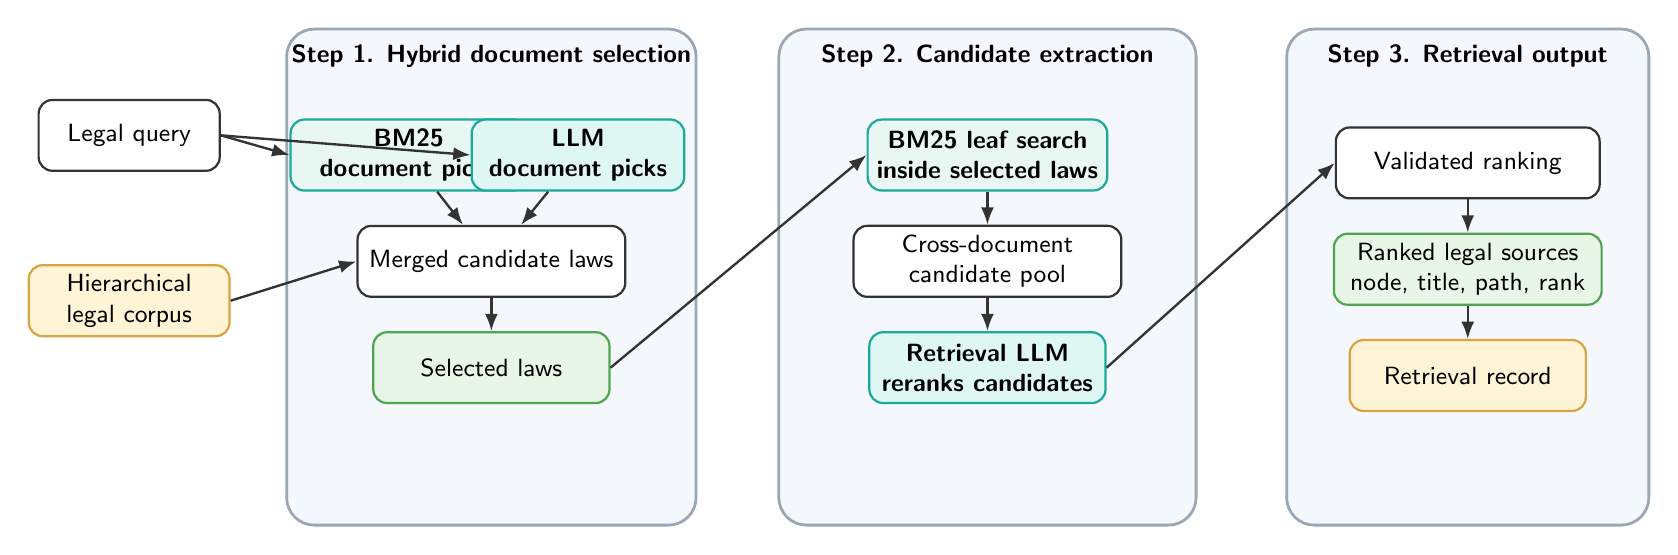
\begin{tikzpicture}

\begin{pgfonlayer}{background}
  \node[panel, minimum width=5.2cm, minimum height=6.3cm] at (4.6, 3.55) {};
  \node[panel, minimum width=5.3cm, minimum height=6.3cm] at (10.9, 3.55) {};
  \node[panel, minimum width=4.6cm, minimum height=6.3cm] at (17.0, 3.55) {};
\end{pgfonlayer}

\node[input] (query) at (0.0, 5.35) {Legal query};
\node[data, minimum width=2.55cm] (corpus) at (0.0, 3.25) {Hierarchical\\legal corpus};

\node[phase-title] at (4.6, 6.35) {Step 1. Hybrid document selection};
\node[score] (bm25doc) at (3.55, 5.1) {BM25\\document picks};
\node[llm, minimum width=2.7cm] (llmdoc) at (5.7, 5.1) {LLM\\document picks};
\node[context] (merge) at (4.6, 3.75) {Merged candidate laws};
\node[output] (docs) at (4.6, 2.4) {Selected laws};

\node[phase-title] at (10.9, 6.35) {Step 2. Candidate extraction};
\node[score] (nodebm25) at (10.9, 5.1) {BM25 leaf search\\inside selected laws};
\node[context] (candidatepool) at (10.9, 3.75) {Cross-document\\candidate pool};
\node[llm] (rerank) at (10.9, 2.4) {Retrieval LLM\\reranks candidates};

\node[phase-title] at (17.0, 6.35) {Step 3. Retrieval output};
\node[context, minimum width=3.35cm] (validated) at (17.0, 5.0) {Validated ranking};
\node[output, minimum width=3.4cm] (sources) at (17.0, 3.65) {Ranked legal sources\\node, title, path, rank};
\node[data, minimum width=3.0cm] (record) at (17.0, 2.3) {Retrieval record};

\draw[flow] (query.east) -- (bm25doc.west);
\draw[flow] (query.east) -- (llmdoc.west);
\draw[flow] (corpus.east) -- (merge.west);
\draw[flow] (bm25doc) -- (merge);
\draw[flow] (llmdoc) -- (merge);
\draw[flow] (merge) -- (docs);
\draw[flow] (docs.east) -- (nodebm25.west);
\draw[flow] (nodebm25) -- (candidatepool);
\draw[flow] (candidatepool) -- (rerank);
\draw[flow] (rerank.east) -- (validated.west);
\draw[flow] (validated) -- (sources);
\draw[flow] (sources) -- (record);

\end{tikzpicture}
\end{document}
